%%%%%%%%%%%%%%%%%%%%%%%%%%%%%%%%%%%%%%%%%%%%%%%%%%%%%
%     Nome: Caio Vinícius Dadauto                   %
%     Número USP(código): 7994808                   %
%     Curso: Laboratório de simulação e computação  %
%     Turma: Noturno                                %
%%%%%%%%%%%%%%%%%%%%%%%%%%%%%%%%%%%%%%%%%%%%%%%%%%%%%

\documentclass [a4paper,10pt]{article}
\newcommand{\n}[1]{\textbf{#1}}
\newcommand{\e}[1]{\textcolor{red}{#1}}
\linespread {1.5}
\usepackage[brazilian]{babel}
\usepackage[utf8]{inputenc}
\usepackage[T1]{fontenc}
\usepackage{amsfonts}
\usepackage{amsmath}
\usepackage{amssymb}
\usepackage{caption}
\usepackage{subcaption}
\usepackage{multirow}
\usepackage{fancyhdr}
\usepackage{graphicx,xcolor}
\usepackage{listings}
\lstset{numbers=left,
stepnumber=1,
firstnumber=1,
numberstyle=\tiny,
extendedchars=false,
breaklines=flase,
tabsize=2,
showtabs=true,
tab=\textcolor{gray}{$\cdots$},
keywordstyle=\color{blue},
frame=tb,
basicstyle=\footnotesize,
stringstyle=\ttfamily,
showstringspaces=false}
\renewcommand{\lstlistingname}{Programa}
\renewcommand{\lstlistlistingname}{Lista de Listagens}
\usepackage[pdftex]{hyperref}
\hypersetup{colorlinks,%
linkcolor=red}

\begin{document}
  \thispagestyle{fancy}
  \fancyhf{}
  \renewcommand{\footrulewidth}{0.0pt}
  \renewcommand{\headrulewidth}{0.0pt}
  \rhead{\bfseries {\scriptsize 13/04/2015}}
  \cfoot{\bfseries \thepage}

  \begin{flushleft}
    \begin{tabular}{ l l }
      \multirow{2}{*}{\rule{0.15\textwidth}{48pt}} & \hspace{-3.5mm}{\large Exercício de Programa 2:}\\[2mm] 
      & \hspace{-3.5mm}{\Huge \n{Método de Monte Carlo}}\\[-3.8mm]
      & \hspace{-4.5mm}\rule{\textwidth}{1.6pt}
    \end{tabular}
  \end{flushleft}
  \begin{center}
    \vspace{-2.5mm}
    \hspace{10mm}{\small\emph{Instituto de Matemática e Estatística da Universidade de São Paulo}}\\[0.5cm]
    \hspace{-5.5cm}\begin{tabular}{ l l }
      \n{Por} & \\[-2mm]
      & \hspace{-10mm}{\small Caio Vinícius Dadauto$\qquad$7994808}\\
      \n{Professor} & \\[-2mm]
      & \hspace{-10mm}{\small Julio Michael Stern}\\[4mm]
    \end{tabular}
  \end{center}
  \vspace{1cm}

  \section{Monte Carlo}
  	Seja a função,
  	\begin{equation}
  		f(t) = 0.25(2^{1.97994808(1-t)})(1 - \sin(0.88084997\pi t));\quad [0, 1]
  	\end{equation}
  	segue métodos implementados para determinar a integral de $f(t)$.
  \subsection{Número de pontos}
  	Para determinar o número de pontos a serem utilizados nos métodos que se seguem,
  	foram gerados números aleatórios distribuidos uniformemente e assim foi feito o
  	desvio padrão da média, ou seja,
  	\begin{equation}
  		\sigma_m = \frac{\sigma}{\sqrt{N}}
  	\end{equation}
  	onde $\sigma = <{f(t)}^2> - {<f(t)>}^2$.
  	
  	Porém, isso garante apenas que há uma prbabilidade de 68\% para que
  	\begin{equation}
  		I_{est} \in [I - \sigma_m, I + \sigma_m]
  	\end{equation}
  	onde $I_{est}$ é a integral estimada pelo método de monte carlo implementado e $I$ a integral de $f(t)$
  	em $[0, 1]$.
  	
  	Assim, buscando um erro de no máximo 0.5\%, estimou-se que o número de pontos gerados aleatóriamente
  	deveriam ser em torno de 200000 pontos.
  	\newpage
  	\pagestyle{fancy}
    \fancyhf{}
    \renewcommand{\footrulewidth}{0.0pt}
    \renewcommand{\headrulewidth}{0.1pt}
    \cfoot{\bfseries \thepage}
    \rhead{\bfseries Exercício de Programa 2}
    \lhead{\setlength{\unitlength}{1mm}
    \begin{picture}(0,0)
	    \put(5,-1){
\includegraphics[scale=0.3]{logo.png}}
    \end{picture}}
    
  \subsection{Cru}
    \begin{equation}
  		I_{est} = \sum_{i = 0}^N f(t_i)
  	\end{equation}
    onde $t_i$ é um número aleatório segundo uma distribuição uniforme e $N$ é o número total de
    parâmetros aleatórios.
    {\linespread{1.15}
    \lstinputlisting[language=octave, label=sqlselect, caption={Implementação para o método Cru}]{cru.m}}
  \subsection{Hit or Miss}
    \begin{equation}
    	I_{est} = \frac{N_0}{N}A
    \end{equation}
    onde $N_0$ são os pontos em uma distribuição uniforme tais que se encontram sobre a região abaixo da funcao
    $f(t)$ (pontos vermelhos em~\ref{hit}) e $A$ é a área limite onde os pontos foram gerados.
	{\linespread{1.15}
    \lstinputlisting[language=octave, label=sqlselect, caption={Implementação para o método Hit or Miss}]{hitmiss.m}}
    \begin{figure}[!ht]
      \centering
      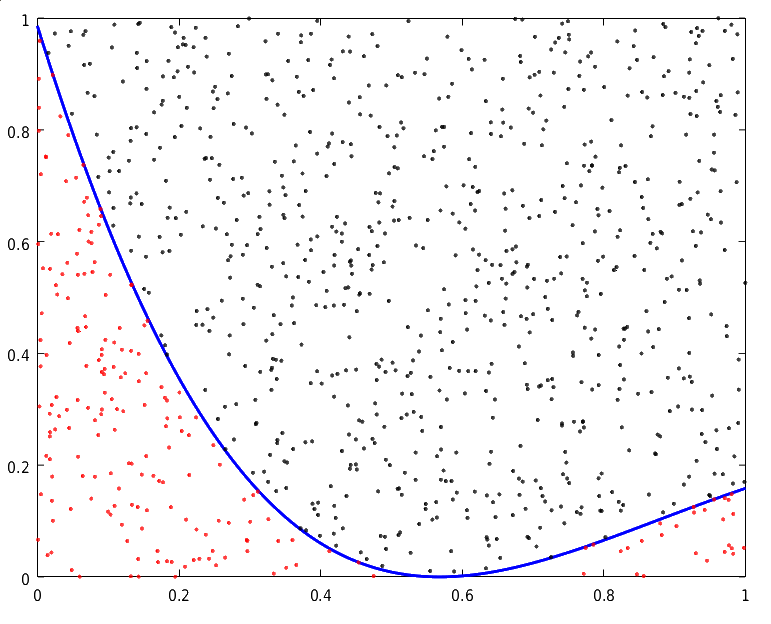
\includegraphics[scale=0.4]{HitMiss.png}
      \caption{Exemplificação do método Hit or Miss.\label{hit}}
    \end{figure}
    
	\subsection{Variavel de controle}
    \begin{equation}
    	I_{est} = \frac{1}{N}\sum_{i = 0}^{N} [f(t_i) - p(t_i] - I_0
    \end{equation}
    onde $p(t)$ é o polinômio de grau dois que melhor aproxima $f(t)$ e $I_0$ é sua integral.
    
    O polinômio foi determinado a partir do método dos mínimos quadrados, pois este se mostrou
    mais adequado que a expansão por \emph{Taylor}, assim como é apresentado na figura \ref{graficos}.
	{\linespread{1.15}
    \lstinputlisting[language=octave, label=sqlselect, caption={Implementação para o método com variável de controle}]{valcont.m}}
    \begin{figure}[!ht]
      \centering
      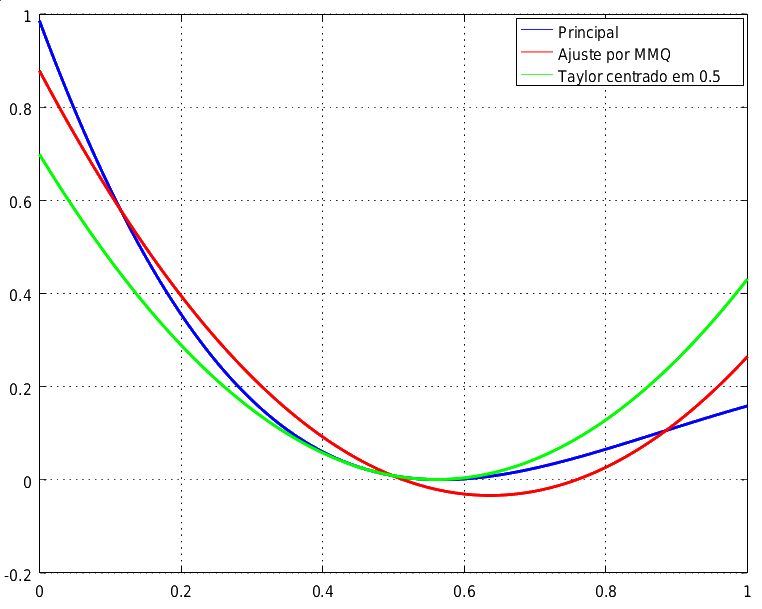
\includegraphics[scale=0.4]{graficos.png}
      \caption{Polinômios ajustados a função $f(t)$.\label{graficos}}
    \end{figure}

	\subsection{Importance Sampling}
    \begin{equation}
    	I_{est} = \frac{1}{N}\sum_{i = 0}^{N}\frac{f(x_i)}{B(x_i)}
    \end{equation}
    onde $B$ é a distrinuição beta que melhor se ajusta afunção $f(t)$. Os parâmetros $x_i$ são obtidos segundo
    a distribuiçaõ beta.
    
    Os parâmetros $\alpha$ e $\beta$ da função beta foram determinados minimizando a disferança da soma dos quadrados
    entre a função beta e a função $f(t)$, como pode ser observado na implementação a seguir.
	{\linespread{1.15}
    \lstinputlisting[language=octave, label=sqlselect, caption={Implementação para o método com variável de controle}]{valcont.m}}
    
    O ajuste e a distribuição dos pontos $x_i$ podem ser observados na seguinte figura:
	  \begin{figure}[!ht]
		\centering
		\begin{subfigure}[!hb]{0.5\textwidth}
		  \centering
		  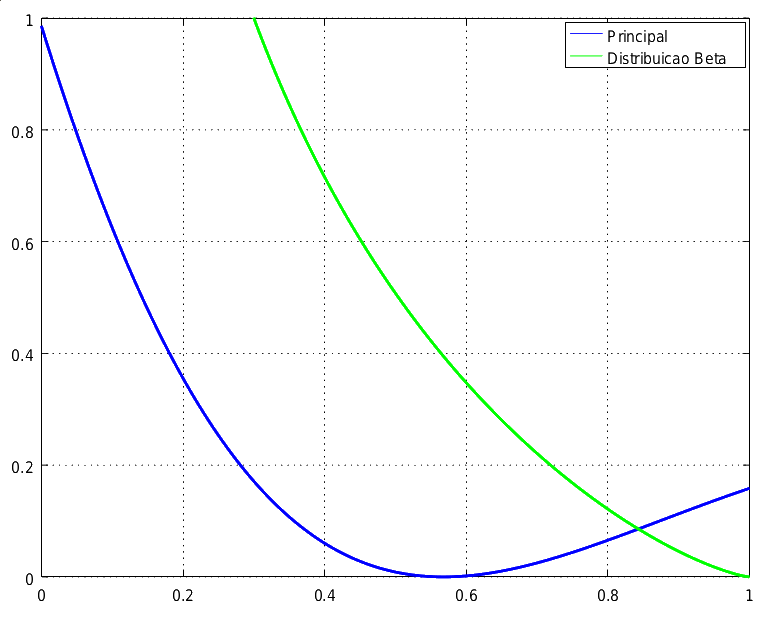
\includegraphics[scale=0.31]{beta.png}
		  \caption{Função beta ajustada.\label{funcaobeta}}
		\end{subfigure}%
		~
		\begin{subfigure}[!hb]{0.5\textwidth}
		  \centering
		  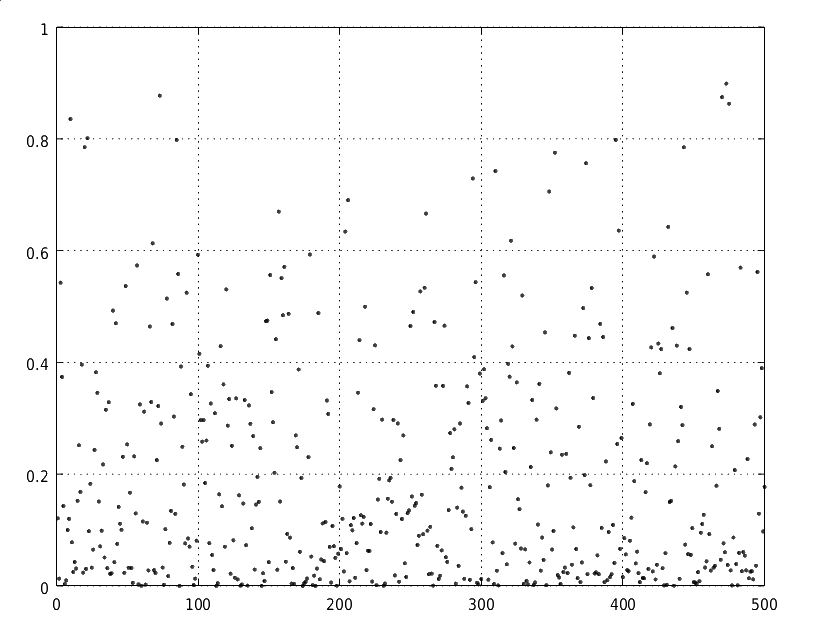
\includegraphics[scale=0.31]{importance.png}
		  \caption{Distribuição beta ajsutada.\label{beta}}
		\end{subfigure}
	  \end{figure}
	  
	\section{Implementação}
	Segue o prgrama completo que retorna como saida alguns dos gráficos apresentados e a estimatima da $I_{est}$ para
	todos os métodos abordados seguido de seus respectivos erros.
	{\linespread{1.15}
    \lstinputlisting[language=octave, label=sqlselect, caption={Implementação final}]{ep2.m}}
\end{document}
